\subsection{Галогенидные комплексы 6 и 10 групп}

\subsubsection*{VI группа}
Для него характерно координационное число 6, что соответсвует октаэдру. МО комплекса $[CrCl_6]^{3-}$:

\begin{figure}[H]
\centering
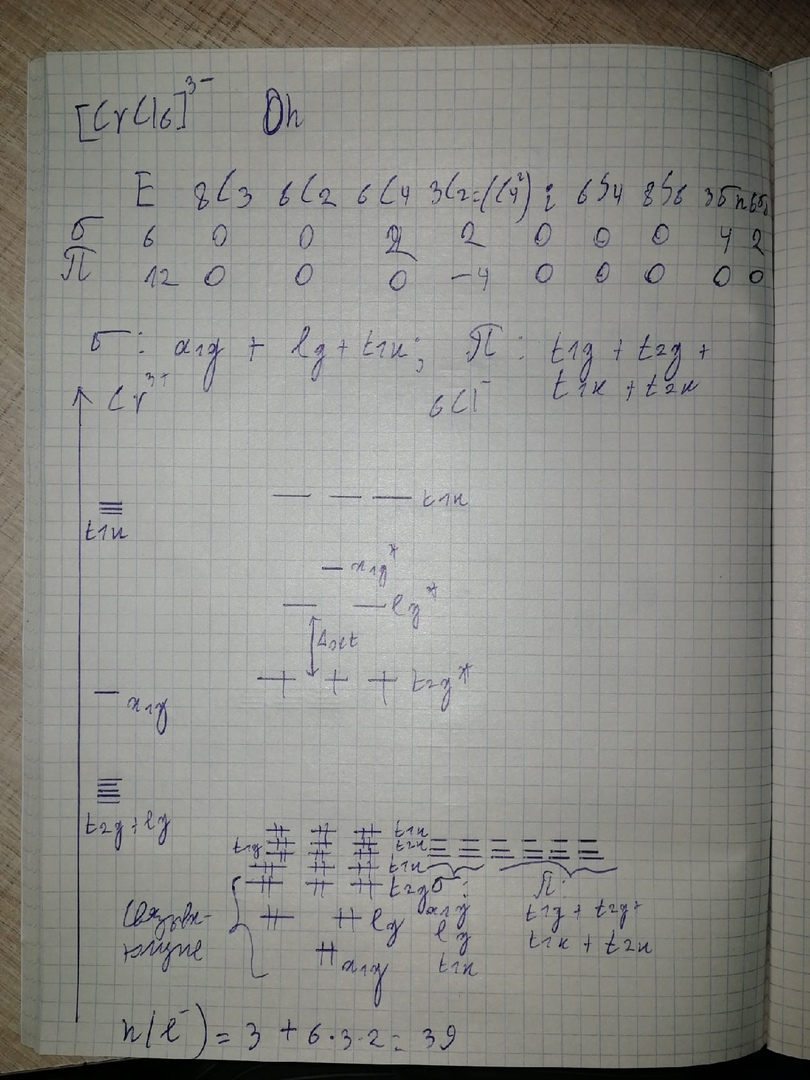
\includegraphics[scale=.300]{images/halogenides.jpg}
\end{figure}

Мы рассматриваем p-орбитали хлора, т.к. на них есть нужные для связывания электроны, связывание может происходить по сигма- и пи-типу.  Орбитали хлора ниже d-орбиталей хрома, т.к. хлор более электроотрицателен. Хорошо бы сравнить результаты с ТКП, которую использоывать сильно проще. Здесь это так и получается, $t_{2g}^*$-орбитали имеют по 1 электрону. Первые заполненные 6 орбиталей связывающие  ПС=(12-3)/2 = 9/2, КС= 9/8 (больше 1, коплекс прочный). 

Магнитный момент, надеюсь, помним, как считать, с этим справитесь. Комплекс окрашен, т.к. щель по энергии маленькая. На это диаграмме видно, почему $Cr^{2+}$ неустойчив, поле слабое и присоединение 1 электрона привело бы к заполнению $e_g^*$-орбиталей, чтего комплексу не очень хочется. Для молибдена и вольфрама ситуация несколько иная. Они сильно выше по энергии, чем хром, в их комплексах поле сильное, они также образуют октаэдры (иногда встречаются тригональные призмы, но это экзотика):

\begin{figure}[H]
\centering
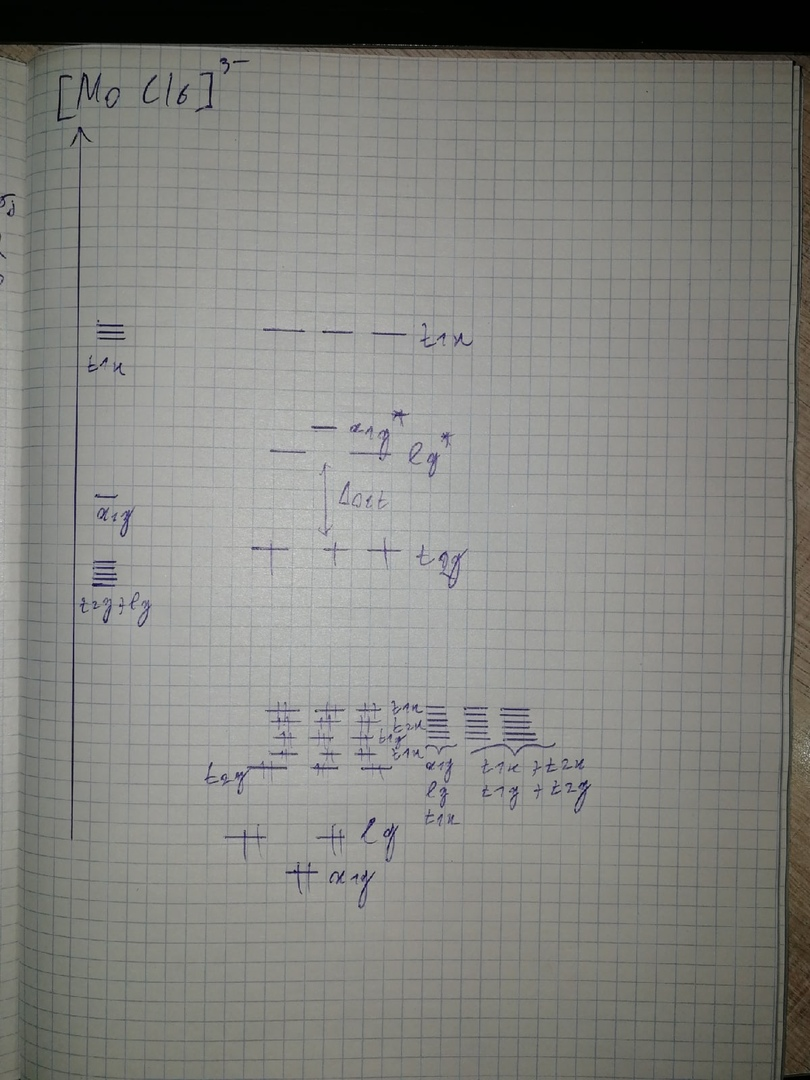
\includegraphics[scale=.300]{images/halogenides2.jpg}
\end{figure}

Симметрия здесь абсолютно такая же. Здесь важно то, что $t_{2g}$ связываются сильно хуже из-за плохого перекрывания, а вот $e_g$, наоборот, очень сильно, что делает расщепление большим. Окрашивания либо совсем нет, либо оно слабое из-за большой энергетической щели. В данно комплексе молибден имеет степень окисления +3, однако орбитали $t_{2g}^*$ лежат довольно высоко. Это объясняет большую склонность молибдена и вольфрама к С.О.=+6, когда разрыхляющие орбитали пусты.

\subsubsection*{X группа}
Здесь комплексы никеля тетраэдрические, поле слабое:

\begin{figure}[H]
\centering
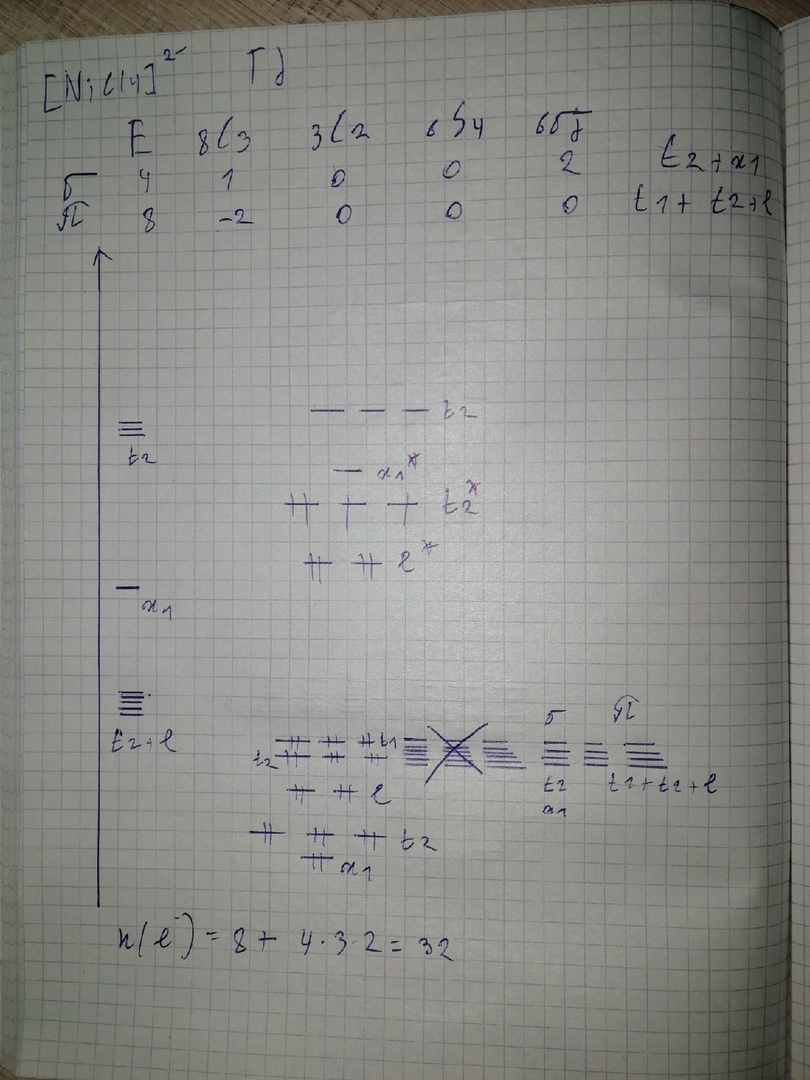
\includegraphics[scale=.300]{images/halogenides3.jpg}
\end{figure}

Здесь лучшее перекрывание с орбиталями $t_2$, хуже – с орбиталями e, что можно увидеть из ТКП. ПС= (12-8)=2, КС=1/2, комплекс не такой прочный. Всё остальное считаем сами, скажу лишь, что он окрашен, т.к. щель маленькая.

\subsubsection*{Палладий и платина}
Комплексы палладия и платины квадратные, поле сильное:

\begin{figure}[H]
\centering
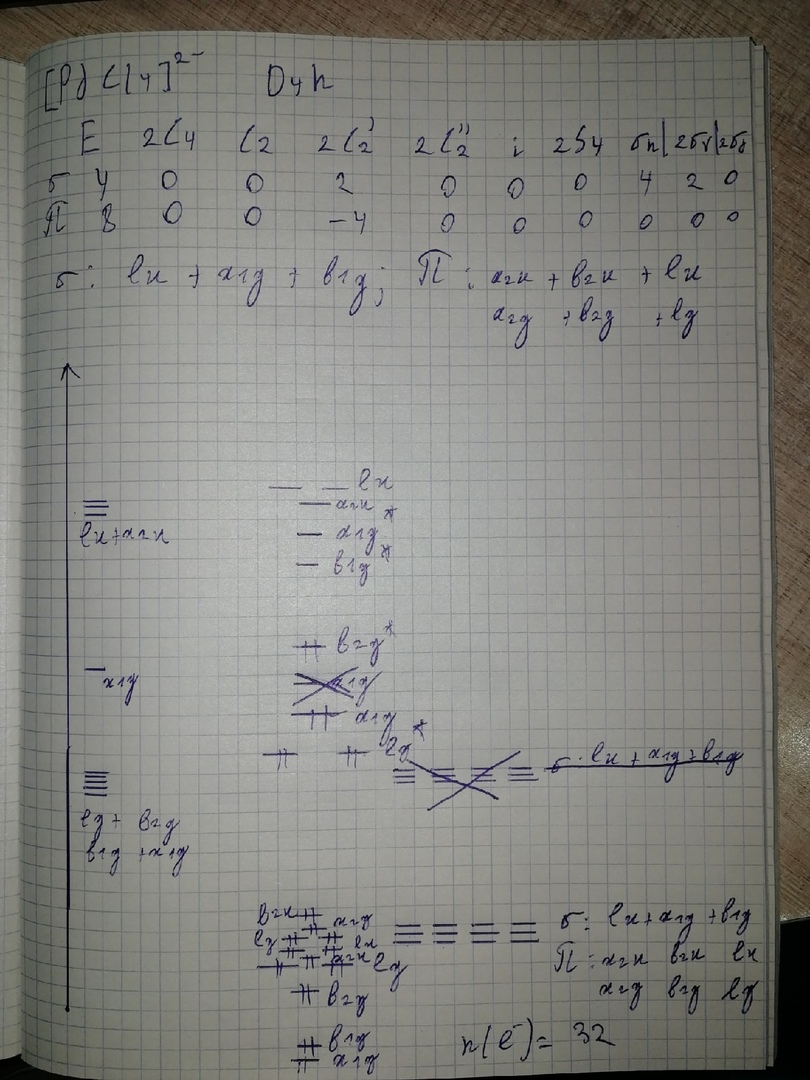
\includegraphics[scale=.300]{images/halogenides4.jpg}
\end{figure}

Здесь следует сказать об орбиталях $a_{1g}$. $s$-орбиталь перекрывается хорошо, даёт связывающую и разрыхляющую. $d_z^2$ даёт существенно несвязывающую. Результат согласуется с ТКП. ПС=(12-6)/2=3, КС = 3/4, что больше, чем в тетраэдрических комплексах, конфигурация металла $d^8$, что соответсвует квадратному расщеплению. Окраски практически нет, диамагнитен.



